%%% Local Variables:
%%% mode: japanese-latex
%%% TeX-engine: uptex
%%% TeX-master: "okuda-master-thesis"
%%% TeX-PDF-mode: t
%%% TeX-PDF-from-DVI: "Dvipdfmx"
%%% End:

\subsection{記号の設定}
本論文の基本的な設定は次のとおりであり,この他に必要な条件は都度明示することとする.

\begin{nttdef}
  \leavevmode\vspace{-1em}
  \begin{itemize}
  \item $\nat,\real, \cpx,\quad$をそれぞれ0を含む自然数全体,実数全体,複素数全体,四元数全体の集合とする.
  \item $G$を非コンパクト実半単純Lie 群,$H$を$G$の非コンパクトな部分Lie群で,$G$のCartan対合$\Theta$に対して$\Theta H = H$なるものとする.
  \item $\ge \defeq \Lie G,\; \ha \defeq \Lie H$とし,$\ge = \ka\oplus \pe$を $\theta \defeq d\Theta$ によるCartan分解とする.
  \item  $e$を$G$の単位元とし,$o_K \defeq eK\in G/K$とする.
  \item $B({-}, {-}) $を$\ge$のKilling形式とし,$\per{\ha}\defeq \{W\in \ge\mid B(W, \ha) = \{0\} \} $とする.
  \item $X\in \pe$に対し,ベクトル空間としての分解$\pe =( \ha\cap \pe)\oplus(\per{\ha}\cap \pe) $に対応した分解を$X = X_1 + X_2 $,$X_1 \in \ha\cap \pe$,$X_2\in \per{\ha}\cap \pe$とする.
  \end{itemize}  
\end{nttdef}

以下の\Cref{thm:kob89-lem6.1}を用いて,$X\in \pe$に対し,$(Y(X), Z(X))\defeq \inv{\pi}(e^X\cdot o_K)\in (\ha\cap\pe)\oplus (\per{\ha}\cap \pe)$と定義する.
\begin{thm}\cite[Lemma~6.1]{kob89}\label{thm:kob89-lem6.1}
  $\pi\colon  (\ha\cap\pe)\oplus (\per{\ha}\cap \pe) \ni (Y, Z)\mapsto e^{Y}e^{Z}\cdot o_K \in G/K $は上への微分同相である.
\end{thm}



ここで,$Y(\real X) $の有界性について,次の\Cref{yosou:1121}が小林俊行氏によって立てられた.
\begin{defi}
  $\pe_{H,\bdd}\defeq \{X\in \pe\mid Y(\real X)\text{ が } \ha\cap \pe \text{ の有界集合である.}  \}  $と定める.
\end{defi}

\begin{yosou}(by T.~Kobayashi)\label{yosou:1121}  
  $\pe_{H,\bdd} = \{X\in \pe\mid [X_1, X_2]\neq 0 \text{ あるいは } X_1 = 0\text{ である.} \}$である.
\end{yosou}

\Cref{yosou:1121}についての基本的な事項を挙げる.

\begin{lem}\label{lem:basic-yosou}
  \leavevmode\vspace{-1em}
  \begin{enumerate}
  \item $\pe_{H,\bdd} \subset \{X\in \pe\mid [X_1, X_2]\neq 0 \text{ あるいは } X_1 = 0 \}$である.
  \item $X \in \pe $が$X_1 = 0$を満たすならば$X\in \pe_{H,\bdd} $である.
  \item 1,2より\Cref{yosou:1121}と「$X\in \pe$が$[X_1,X_2]\neq 0$ならば$X\in \pe_{H,\bdd} $である」は同値である.
  \item $G$が実階数1のとき,\Cref{yosou:1121}と「$\pe_{H,\bdd} =  \{0\}\cup \pe\setminus\ha $」は同値である.
  \end{enumerate}
\end{lem}

\begin{pfwn}{\Cref{lem:basic-yosou}}
  \leavevmode
  \vspace{-2em}
  \begin{enumerate}
  \item 背理法による.$[X_1,X_2 ] = 0$かつ$X_1\neq 0$なる$X  \in \pe $に対しては$[X_1,X_2 ] = 0$より$e^{tX_1}e^{tX_2}\cdot o_K = e^{t(X_1 + X_2)}\cdot o_K = e^{tX}\cdot o_K$である.したがって\Cref{thm:kob89-lem6.1}より$Y(tX) = tX_1 $,$Z(tX) = tX_2 $であることから$Y(\real X) = \real X_1 $となり,$X_1\neq 0$より$Y(\real X)$は有界集合とならない.
  \item $X_1 = 0\iff X\in \per{\ha}\cap\pe $より$Z(tX) = tX $,$Y(tX) = 0 $であることによる.
  \item[4.] 同値な命題である「$X\in \pe$に対し,$[X_1,X_2] = 0 $かつ$X_1 \neq 0$であることと$f X \in \ha\setminus\{0\} $であることは同値である」を示せば良い.$G$の実階数は1で,$H$は非コンパクトかつ$\Theta H = H$であるから,$\ha\subset \pe$であり,$\ha$は$\ge$の極大可換部分空間である.よって$X_1\neq 0$かつ$[X_1,X_2] = 0  \implies X_2 = 0 $であり,$X = X_1 + X_2\in \ha\setminus\{0\} $を得る.
  \end{enumerate}
  
\end{pfwn}

$Y(\real X) $の有界性は$\Ad(k) $-不変である.つまり\Cref{lem:1101}が成り立つ.
\begin{lem}\label{lem:1101}
  $k\in K$,$X\in \pe$に対し,$X'\defeq \Ad(k)X $,$\ha'\defeq \Ad(k)\ha $とする.$Y'(X'), Z'(X') $を,微分同相$\pi'\colon (\ha'\cap \pe)\oplus (\per{\ha'}\cap \pe)\ni (Y',Z')\mapsto e^{Y'}e^{Z'}\cdot o_K  $を用いて,$X'\in \pe$に対し,$(Y'(X'), Z'(X')) = \inv{\pi'}(e^{X'}\cdot o_K) $と定めると,$Y(\real X)$が有界$\iff Y'(\real X') $が有界である.
\end{lem}

\begin{pfwn}{\Cref{lem:1101}}

  主張は$(X,\ha) $と$(X',\ha')$に対して対称的であるから,$Y(\real X) $が有界ならば$Y'(\real X') $が有界であることのみを示せば十分である.

  任意に$r\in \real$を取る.$e^{rX'}\cdot o_K = e^{Y'(r X')}e^{Z'(r X')}\cdot o_K  $であり,両辺に左から$\inv{k} $を掛けると,$e^{r X} = e^{\Ad(\inv{k})( Y'(r X'))}e^{\Ad(\inv{k})( Z'(r X'))}\cdot o_K  $を得る.ここで$Y'(rX')\in \ha'\cap \pe $,$Z'(r X')\in \per{\ha'}\cap \pe $であるから$\Ad(\inv{k})(Y'(r X'))\in \ha\cap \pe $,$\Ad(\inv{k})(Z'(r X')) \in \per{\ha}\cap \pe $である.

  \Cref{thm:kob89-lem6.1}により$\pi$は微分同相であるから任意の$r\in \real$に対して$\Ad(\inv{k})(Y'(r X')) = Y(rX)  $である.$Y'(\real X) = \Ad(k)(Y(\real X))  $であり,$\Ad(k) $は有限次元空間の間の線型写像であるから有界性を保つ.

  以上から\Cref{lem:1101}が示された.
  
\end{pfwn}


$Z(\real X) $の有界性については次の定理が知られており,有界性の判定はLie環の言葉のみで行える.

\begin{thm}\cite[Lemmma~5.4]{kob97}\label{thm:kob97}  
  $X\in \pe$に対し,$\norm{Z(X)}\geq \norm{X} \sin\phi(X, \ha\cap\pe)$である.

  ここに$\phi(X,\ha\cap \pe) $は$X$と$\ha\cap \pe$の元がなす角度の最小値$0\leq \phi(X,\ha\cap \pe) \leq \frac{\pi}{2} $であり,
  $X\in \pe\setminus \ha \iff \phi(X,\ha\cap \pe)\neq 0 $である.
\end{thm}

つまり$ X\in \pe\setminus \ha$ならば$\norm{Z(t X)}\to \infty $,$\abs{t}\to \infty $である.


\subsection{\Cref{yosou:1121}の観察: $G = \SU(1,1) $,$H = \SO(1,1) $の場合}

$G = \SU(1,1) $,$H = \SO(1,1) \defeq\lbig\{
\begin{pmatrix}
  \cosh t & \sinh t\\ \sinh t & \cosh t
\end{pmatrix}
\relmiddle| t\in \real \rbig\} $の場合に\Cref{yosou:1121}が正しいことは直接計算により確かめられる.

\begin{prop}\label{prop:yosou-eg}
  $G = \SU(1,1) $,$H = \SO(1,1) $のとき\Cref{yosou:1121}は正しい.
\end{prop}

% \bluetext{$\sulie(1,1) $のKilling形式と$r = \tanh t$の関係を明記せよ.}

\begin{lem}\label{lem:riem-metric-su11}
  $\ge\defeq \sulie(1,1)$のKilling形式から定まる{\Poincare}円板$G/K =\{x+\sqrt{-1}y\mid x^2 + y^2 < 1 \} $の計量は$ \dfrac{8(dx^2 + dy^2)}{(1 - x^2 - y^2)^2} $である.
\end{lem}

\begin{pfwn}{\Cref{lem:riem-metric-su11}}
  
$\ge$の元を$G/K$上の左不変ベクトル場と同一視すると$X' \defeq 
\begin{pmatrix}
  0 & 1 \\ 1 & 0
\end{pmatrix} = \dfrac{\del}{\del x}
$,$Y' \defeq 
\begin{pmatrix}
  0 & \sqrt{-1} \\ -\sqrt{-1} & 0
\end{pmatrix} = \dfrac{\del}{\del y}
$である.$\ge$のKilling形式$B$から定まる$\pe$上のノルム$\norm{-} $に対して$\norm{X'}^2 = \norm{Y'}^2 = 8 $,$B(X', Y' ) = 0$であって,$0\in G/K =\{x+\sqrt{-1}y\mid x^2 + y^2 < 1 \}  $で主張が成り立つ.

したがって$k_{\theta} \defeq \diag(e^{\sqrt{-1}\theta},e^{-\sqrt{-1}\theta}) $,$a_r\defeq
\begin{pmatrix}
  \cosh r & \sinh r \\  \sinh r & \cosh r
\end{pmatrix}
$とすると,
\begin{align*}
  &g(d\tau(k_{\theta/2}a_r)(d\tau(k_{-\theta/2})X'), d\tau(k_{\theta/2}a_r)(d\tau(k_{-\theta/2})X')) \\
  =&\ g (d\tau(k_{\theta/2}a_r)(d\tau(k_{-\theta/2})Y'), d\tau(k_{\theta/2}a_r)(d\tau(k_{-\theta/2})Y')) \\
  =&\ 8, \\
  &g(d\tau(k_{\theta/2}a_r)(d\tau(k_{-\theta/2})X'), d\tau(k_{\theta/2}a_r)(d\tau(k_{-\theta/2})Y'))  = 0
\end{align*}
なるような計量$g $がKilling形式から誘導される計量であるが,それが主張の形であることを示せば良い (これらのベクトルが何を表しているかは\Cref{fig:riem-metric-su11}参照).

\begin{figure}[H]
  \centering
  % \raggedleft
  % \raggedrightp
  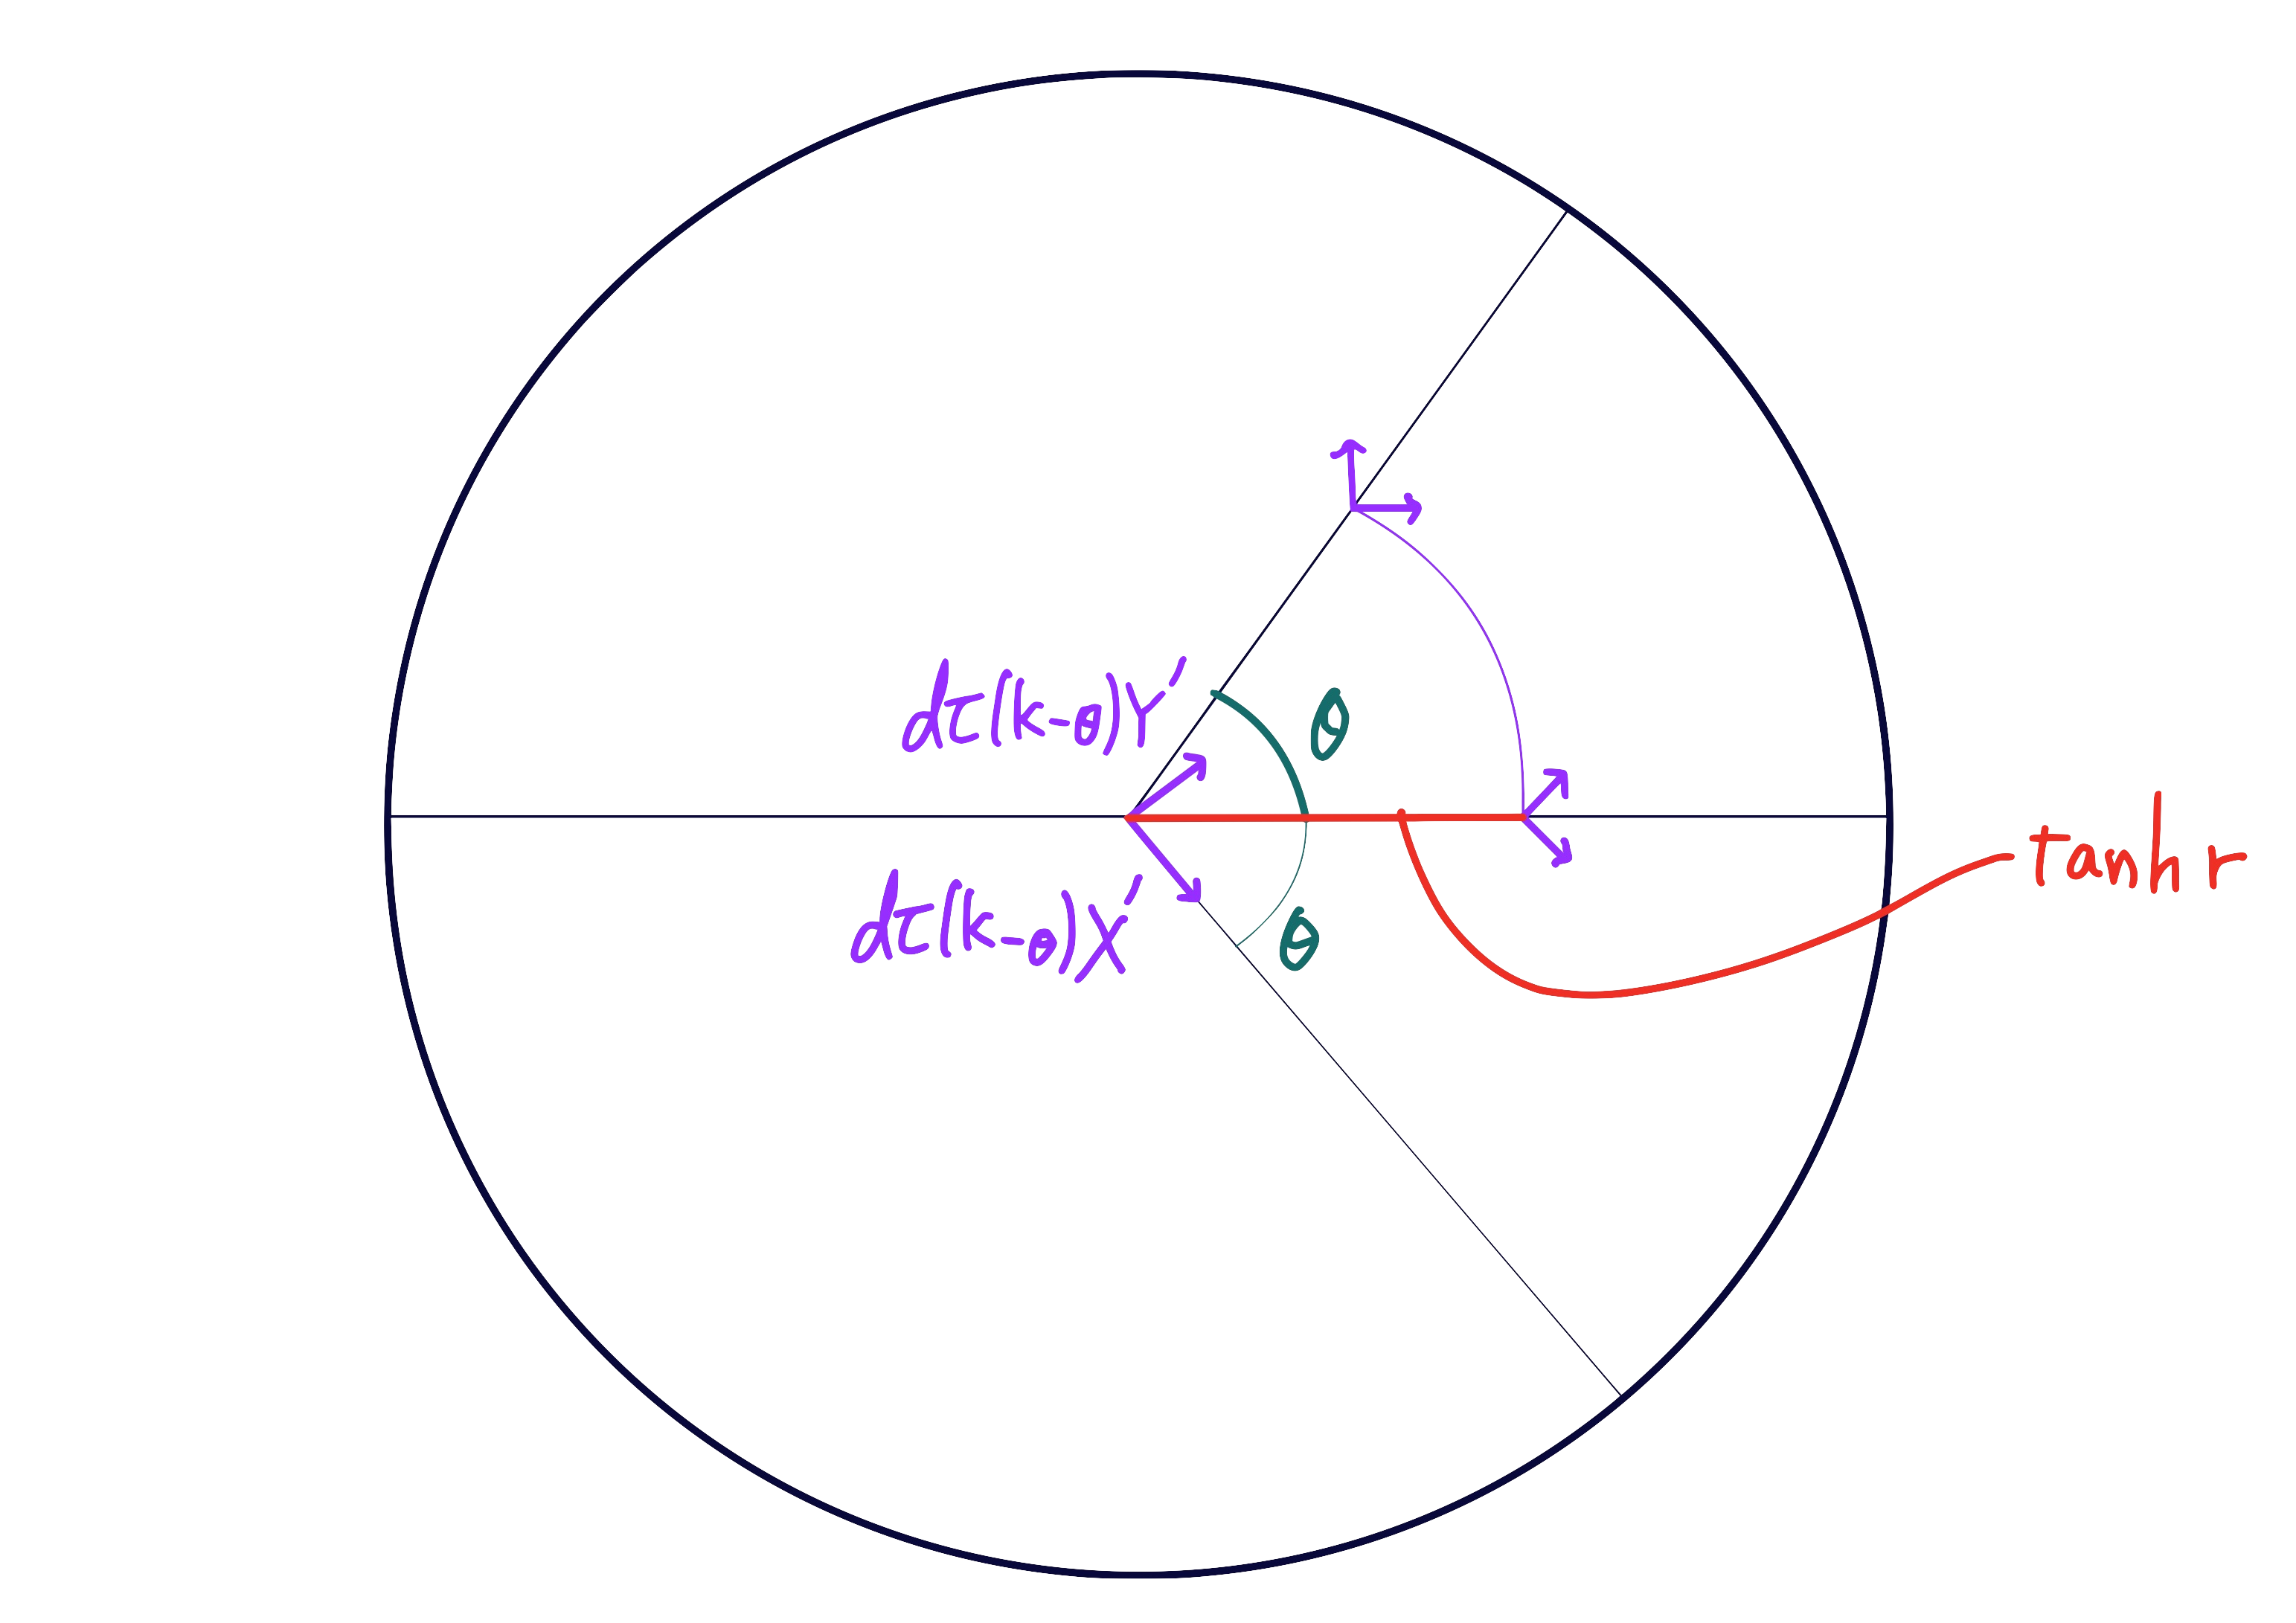
\includegraphics[scale=0.08]{../graph/riem-su11.png}
  % 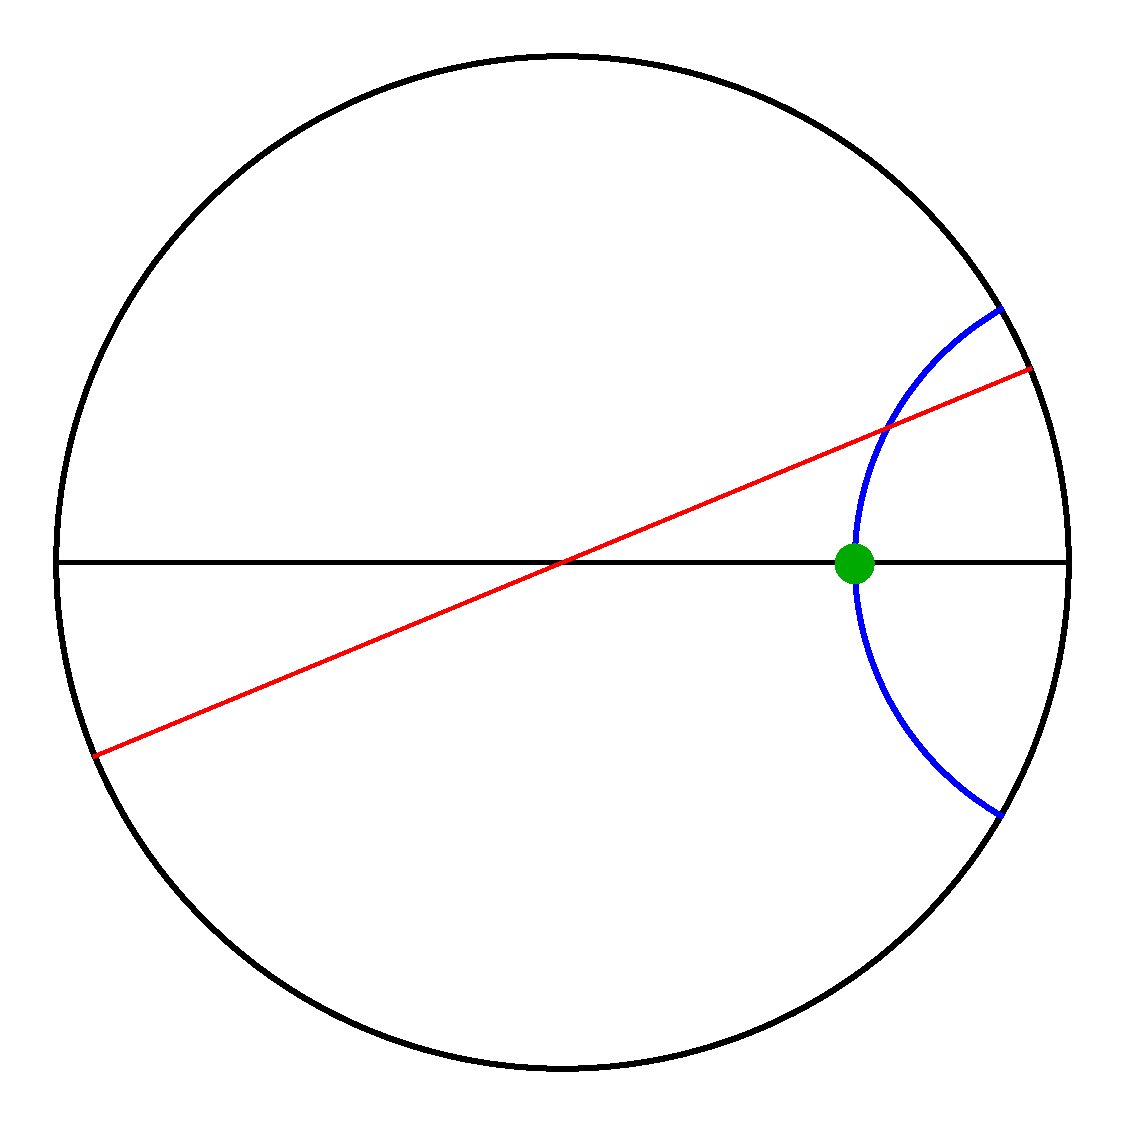
\includegraphics[scale=0.3]{../graph/y-and-z.pdf}
  \caption{}
  \label{fig:riem-metric-su11}
\end{figure}


$t = 0$での接ベクトルが$d\tau(k_{\theta/2}a_r)d\tau(k_{-\theta/2})X'$を与える曲線は
\begin{align*}
  \gamma_x(t) \defeq  e^{\sqrt{-1} \theta}\dfrac{\cosh r\cdot e^{-\sqrt{-1}\theta} \tanh t + \sinh r }{\sinh r\cdot e^{-\sqrt{-1}\theta} \tanh t + \cosh r}
\end{align*}
であるから,
\begin{align*}
  \lbig.\dfrac{d}{dt}\rbig|_{t=0}\gamma_x(t) = d\tau(k_{\theta/2}a_r)d\tau(k_{-\theta/2})X' = (1 - \tanh^2 r)\dfrac{\del}{\del x} = (1-x^2-y^2)\dfrac{\del}{\del x}
\end{align*}
である.

同様に$t = 0$での接ベクトルが$d\tau(k_{\theta/2}a_r)d\tau(k_{-\theta/2})Y'$を与える曲線は
\begin{align*}
\gamma_y(t) \defeq  e^{\sqrt{-1} \theta}\dfrac{\cosh r\cdot e^{-\sqrt{-1}\theta}\sqrt{-1} \tanh t + \sinh r }{\sinh r\cdot e^{-\sqrt{-1}\theta}\sqrt{-1} \tanh t + \cosh r}
\end{align*}
であるから,
\begin{align*}
\lbig.\dfrac{d}{dt}\rbig|_{t=0}\gamma_y(t) = d\tau(k_{\theta/2}a_r)d\tau(k_{-\theta/2})Y' = (1 - \tanh^2 r)\dfrac{\del}{\del y} = (1-x^2-y^2)\dfrac{\del}{\del y}
\end{align*}
である.

以上より$g  =  \dfrac{8(dx^2 + dy^2)}{(1 - x^2 - y^2)^2} $が示された.

\end{pfwn}


\begin{pfwn}{\Cref{prop:yosou-eg}}


  $k_{\theta} \defeq \diag(e^{\sqrt{-1}\theta},e^{-\sqrt{-1}\theta}) $,$X_{\theta} \defeq k_{\theta/2}
  \begin{pmatrix}
    0 & 1 \\ 1 & 0
  \end{pmatrix}
  k_{-\theta/2}$とすると,$\pe\setminus\{0\} =  \{tX_{\theta}\mid t\in \real_{>0},\ 0\leq \theta\leq \pi\}$である.この$X_{\theta} $と$t\in \real$に対して$Y(tX_{\theta} ) = s
  \begin{pmatrix}
    0 & 1 \\ 1 & 0
  \end{pmatrix}
  $なる$s\in \real $を求める.


   
  \begin{figure}[H]
    \centering
    % \raggedleft
    % \raggedrightp
    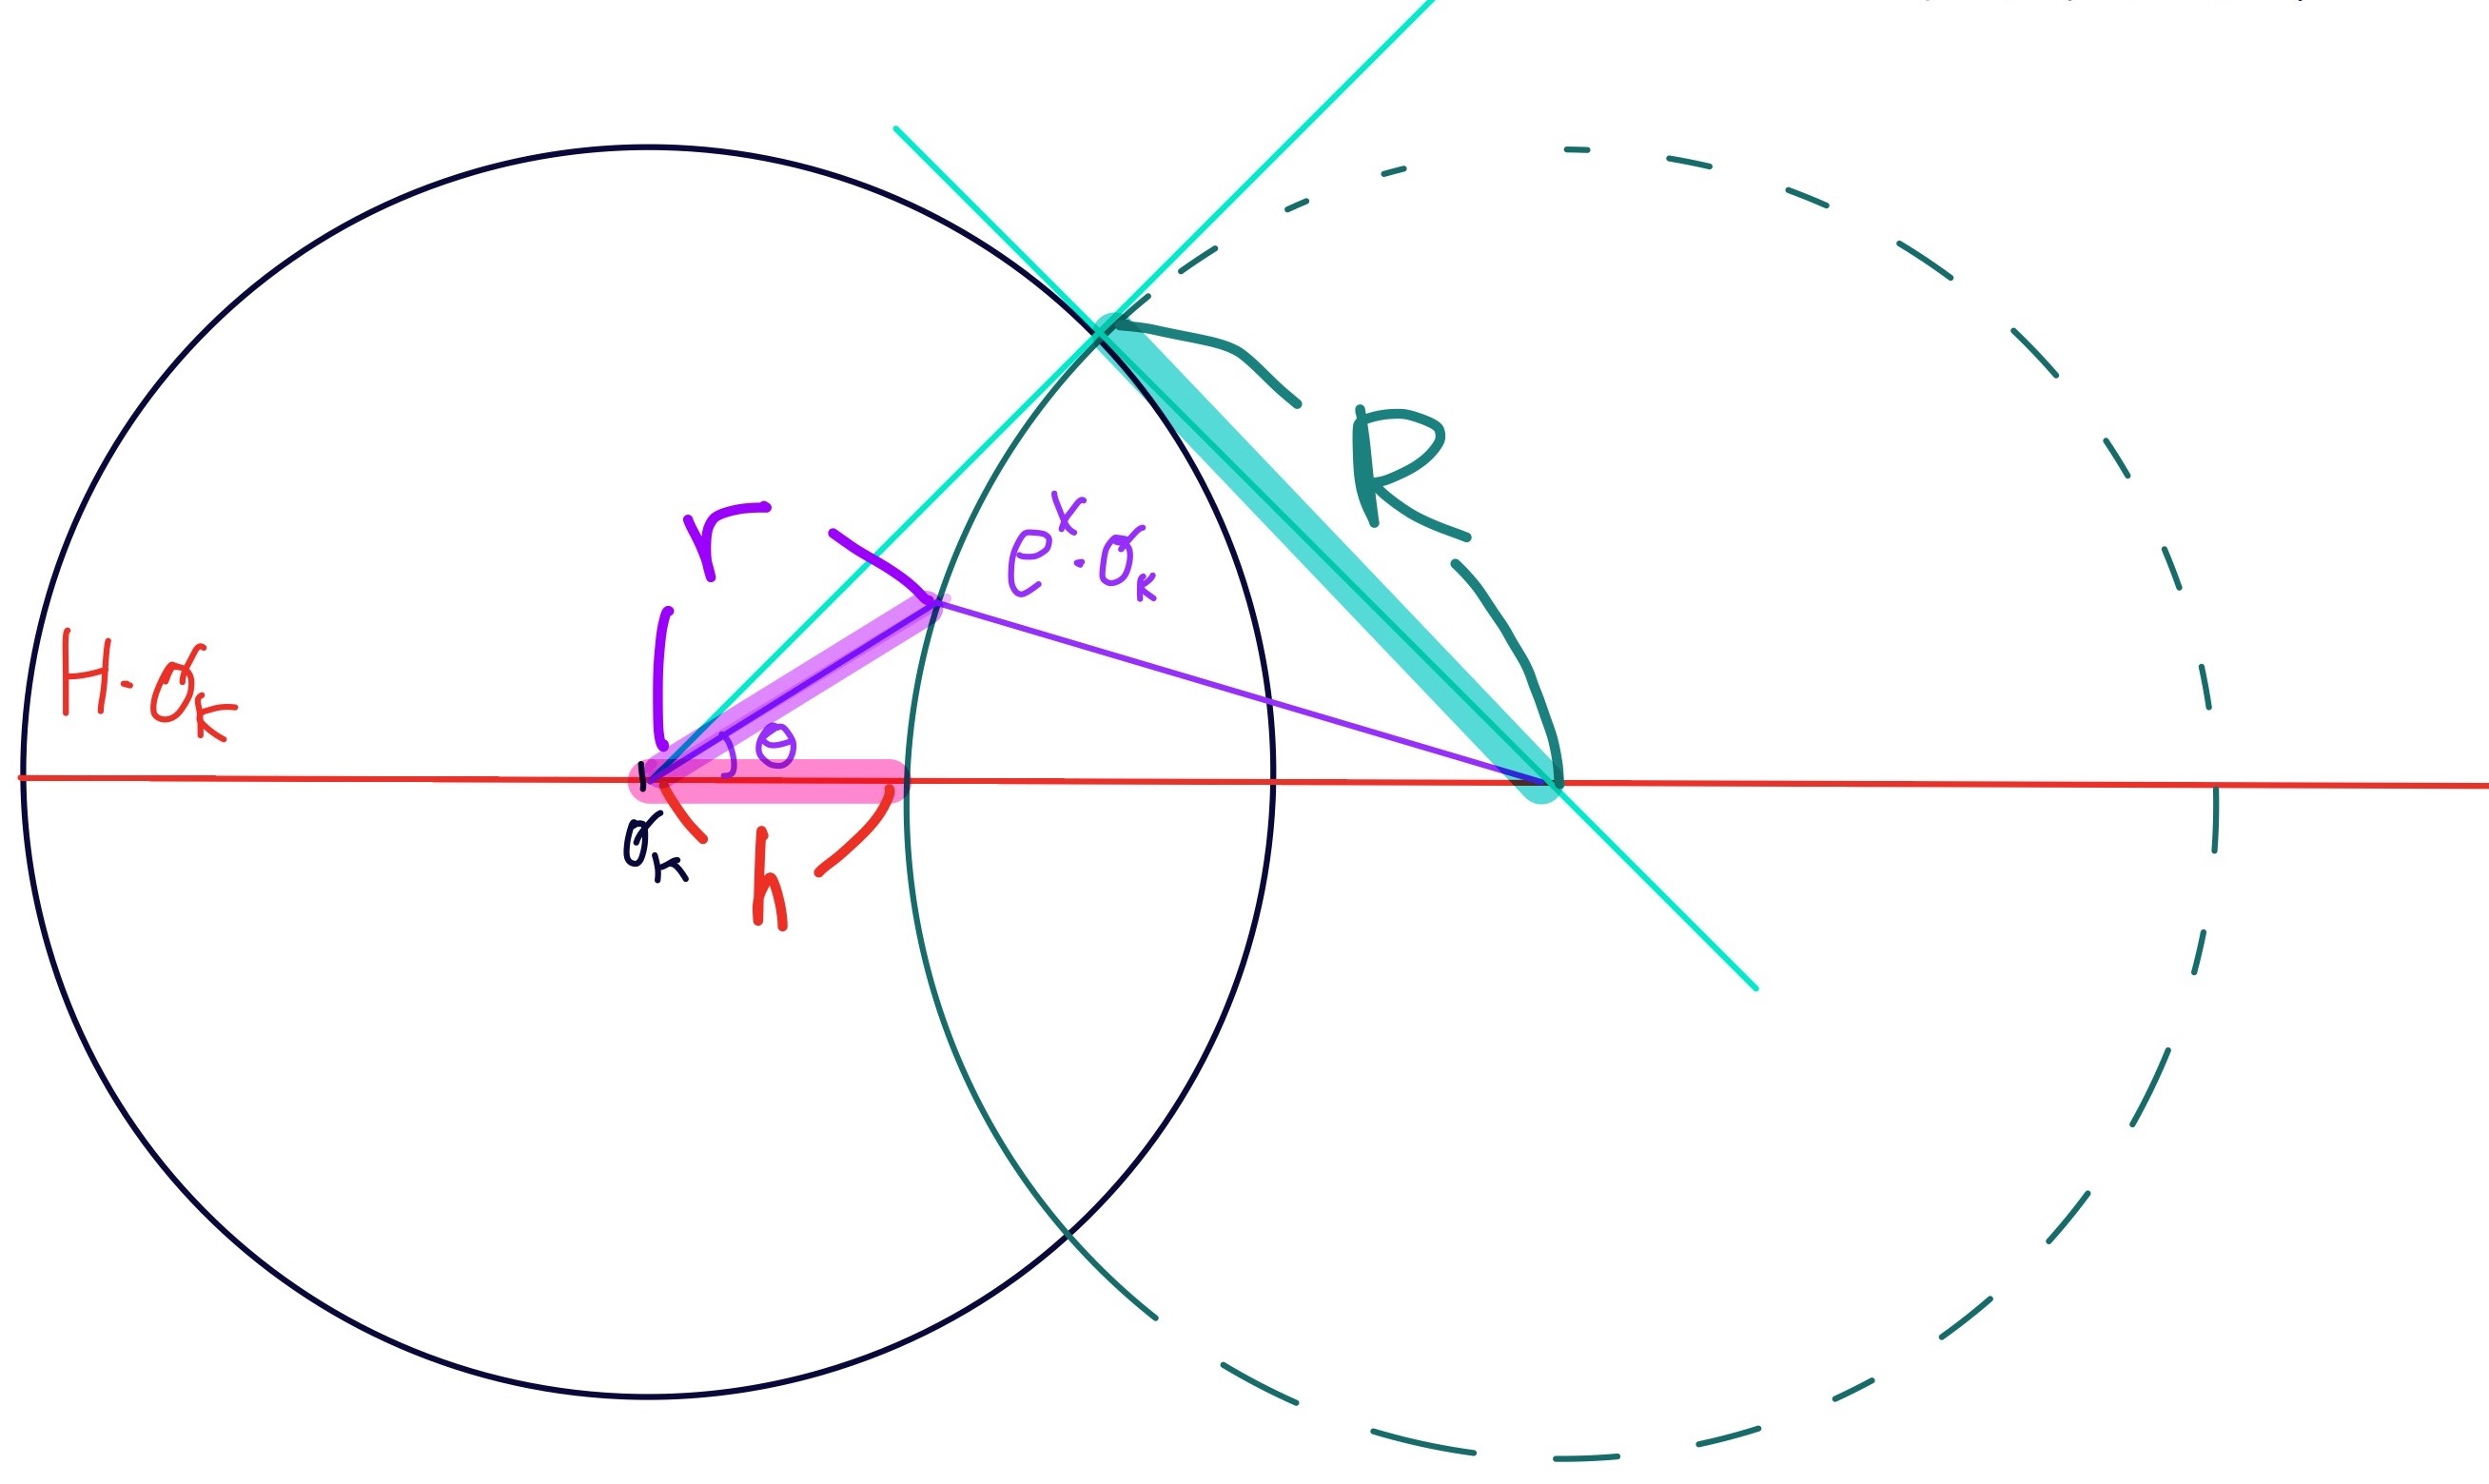
\includegraphics[scale=0.08]{../graph/yosou-eg-1.jpg}
    % 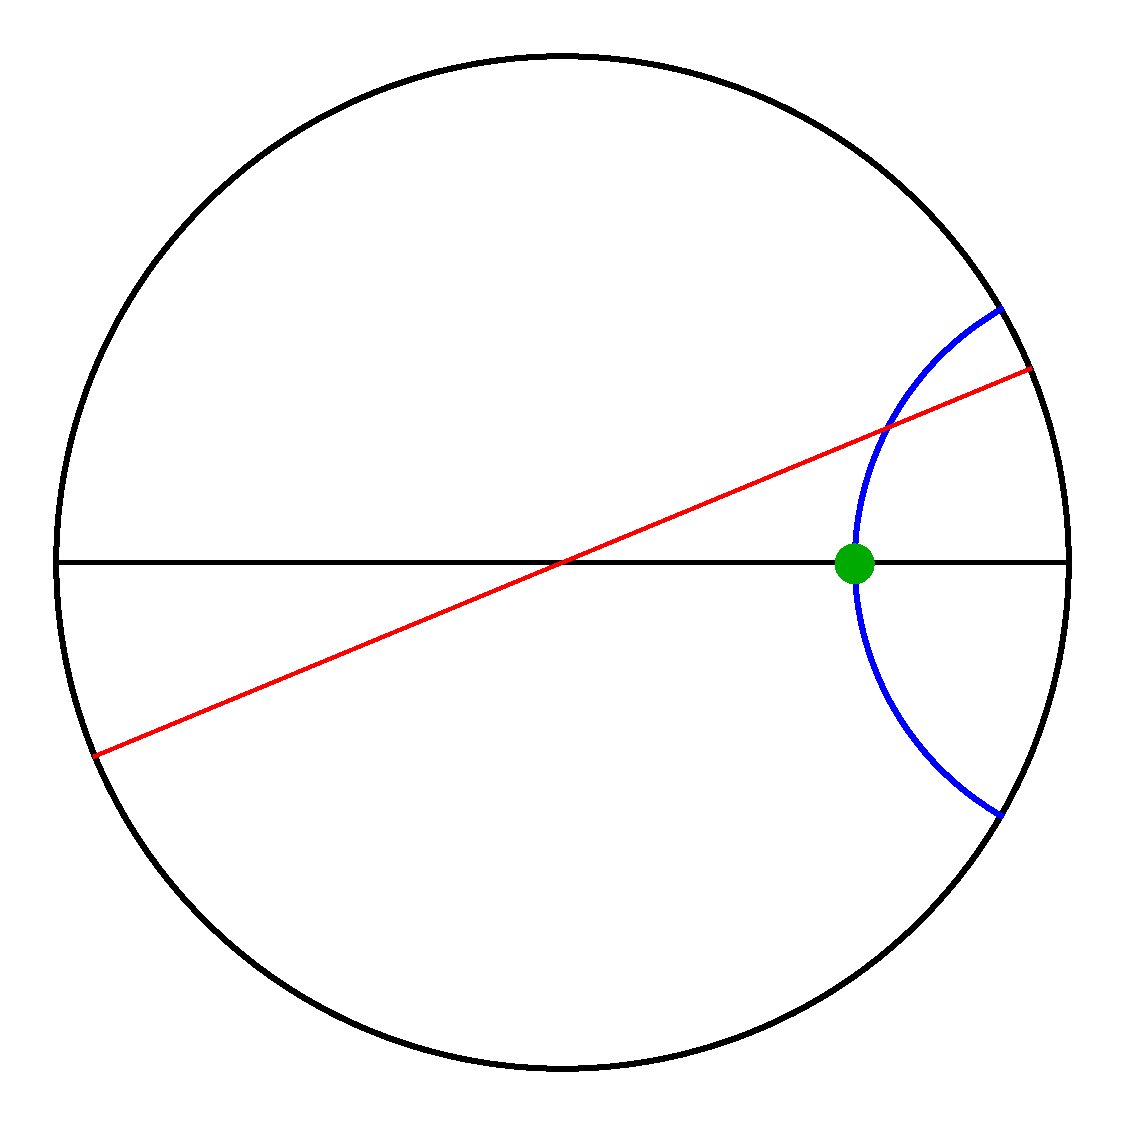
\includegraphics[scale=0.3]{../graph/y-and-z.pdf}
    \caption{}
    \label{fig:yosou-eg-1}
  \end{figure}

  右の円の Euclid 距離での半径を$R$とし,$e^{tX_{\theta}}\cdot o_K $から$H\cdot o_K$への垂線の足の$o_K$からの Euclid 距離を$h$とするとき,外側の青色の直角三角形に対して三平方の定理を用いて$(h+R)^2 = R^2 +  1 $より$R = \frac{1-h^2}{2h} , R+h = \frac{1+h^2}{2h}  $を得る.

  さらに下の紫色の三角形に対して余弦定理を用いて$R^2 = (R+h)^2 + r^2 - 2(R+h) \cos\theta  $を得,
  \begin{align}
    {\dfrac{2r\cos\theta}{r^2 + 1} = \dfrac{2h}{h^2 + 1} }\label{eq:1018-main}
  \end{align}
  を得る.

  \bluetext{要確認: ここで\Cref{lem:riem-metric-su11}より$\dfrac{r}{2\sqrt{2}} = \tanh {2\sqrt{2}}t$,$\dfrac{h}{2\sqrt{2}} = \tanh {2\sqrt{2}}s$であり\Cref{eq:1018-main} は$\cos\theta \tanh \dfrac{t}{4\sqrt{2}} = \tanh \dfrac{s}{4\sqrt{2}} $と書き直せる.したがって$X_{\theta}$に対して$Y(\real X) $が有界$\iff \abs{\cos\theta}\neq 1 \iff  X\nin \ha  $である.}
  
\end{pfwn}

\begin{rem}\label{rem:su11-by-angle}

  \Cref{prop:yosou-eg}は角度を用いた議論によっても示すことができる.具体的には,計算により次の\Cref{lem:0106}が示せる.
  \begin{lem}\label{lem:0106}
    $e^{tY}e^{s Z}\cdot o_K =
    \begin{pmatrix}
      \cosh t & \sinh t\\ \sinh t & \cosh t
    \end{pmatrix}
    \sqrt{-1}\tanh s \in \SU(1,1)/\U(1) $,$t > 0$,$s\in \real$に対し,$o_K $と$e^{tY}e^{sZ}\cdot o_K$を結ぶ測地線が$o_K$と$e^{tY}\cdot o_K $を結ぶ測地線と$o_K$でなす角$\phi_{s,t} $は,$\tan \phi_{s,t} = \dfrac{\tanh 2s}{\sinh 2t} $を満たす.
  \end{lem}
  ただし,$Y \defeq
  \begin{pmatrix}
    0 & 1\\ 1 & 0
  \end{pmatrix}
  $,$Z \defeq \begin{pmatrix}
    0 & \sqrt{-1} \\ -\sqrt{-1} & 0
  \end{pmatrix}$とする.

  \Cref{lem:0106}により\Cref{prop:yosou-eg}は次のように証明できる.
  任意の$s\in \real, 0\neq t\in \real $に対し,
  \begin{align*}
    \lim_{s\to -\infty}\tan \phi_{s,\abs{t}} = \dfrac{-1}{\sinh 2\abs{t}}  \leq \tan \phi_{s,t} \leq  \lim_{s\to \infty}\tan \phi_{s,\abs{t}} = \dfrac{1}{\sinh 2\abs{t}}
  \end{align*}
  であるから,$X\nin \real Y $の元に対して$Y(\real X) $が非有界であるとすると,$\phi(X,\ha) >  \epsilon > 0$なる$\epsilon$に対し,ある$r\in \real $が存在して,$Y(rX) = tY $,$Z(rX) = sZ $に対し$\abs{\tan \phi_{s,t}} < \tan \epsilon $となり,$o_K$と$e^{tY}e^{sZ}\cdot o_K$を結ぶ測地線が$o_K$と$e^{tY}\cdot o_K $を結ぶ測地線と$o_K$でなす角が$\epsilon$未満,つまり$\ha$と$X$の角度未満となって矛盾する ($o_K$と$e^{tX}\cdot o_K (= e^{tY}e^{sZ}\cdot o_K)  $を結ぶ測地線が$o_K$と$e^{tY}\cdot o_K $を結ぶ測地線と$o_K$でなす角は$\phi(X,\ha)$である).

  
\end{rem}

\begin{cor}\label{cor:yosou-eg}
  $G = \SO(1,n) $,$H = \SO(1,k) $,$1\leq k\leq n-1$に対して\Cref{yosou:1121}は正しい.
\end{cor}


\begin{pfwn}{\Cref{cor:yosou-eg}}
  $\SO(1,n)/\SO(n)$の開球としての実現を考える.「$e^X\cdot o_K $と$o_K$を結ぶ直線」と$H\cdot o_K$で張られる超平面で$\SO(1,n)/\SO(n)$を切った際の断面を考える.
  \begin{figure}[H]
    \centering
    % \raggedleft
    % \raggedrightp
    % \includegraphics[scale=0.08]{../graph/fig1.jpg}
    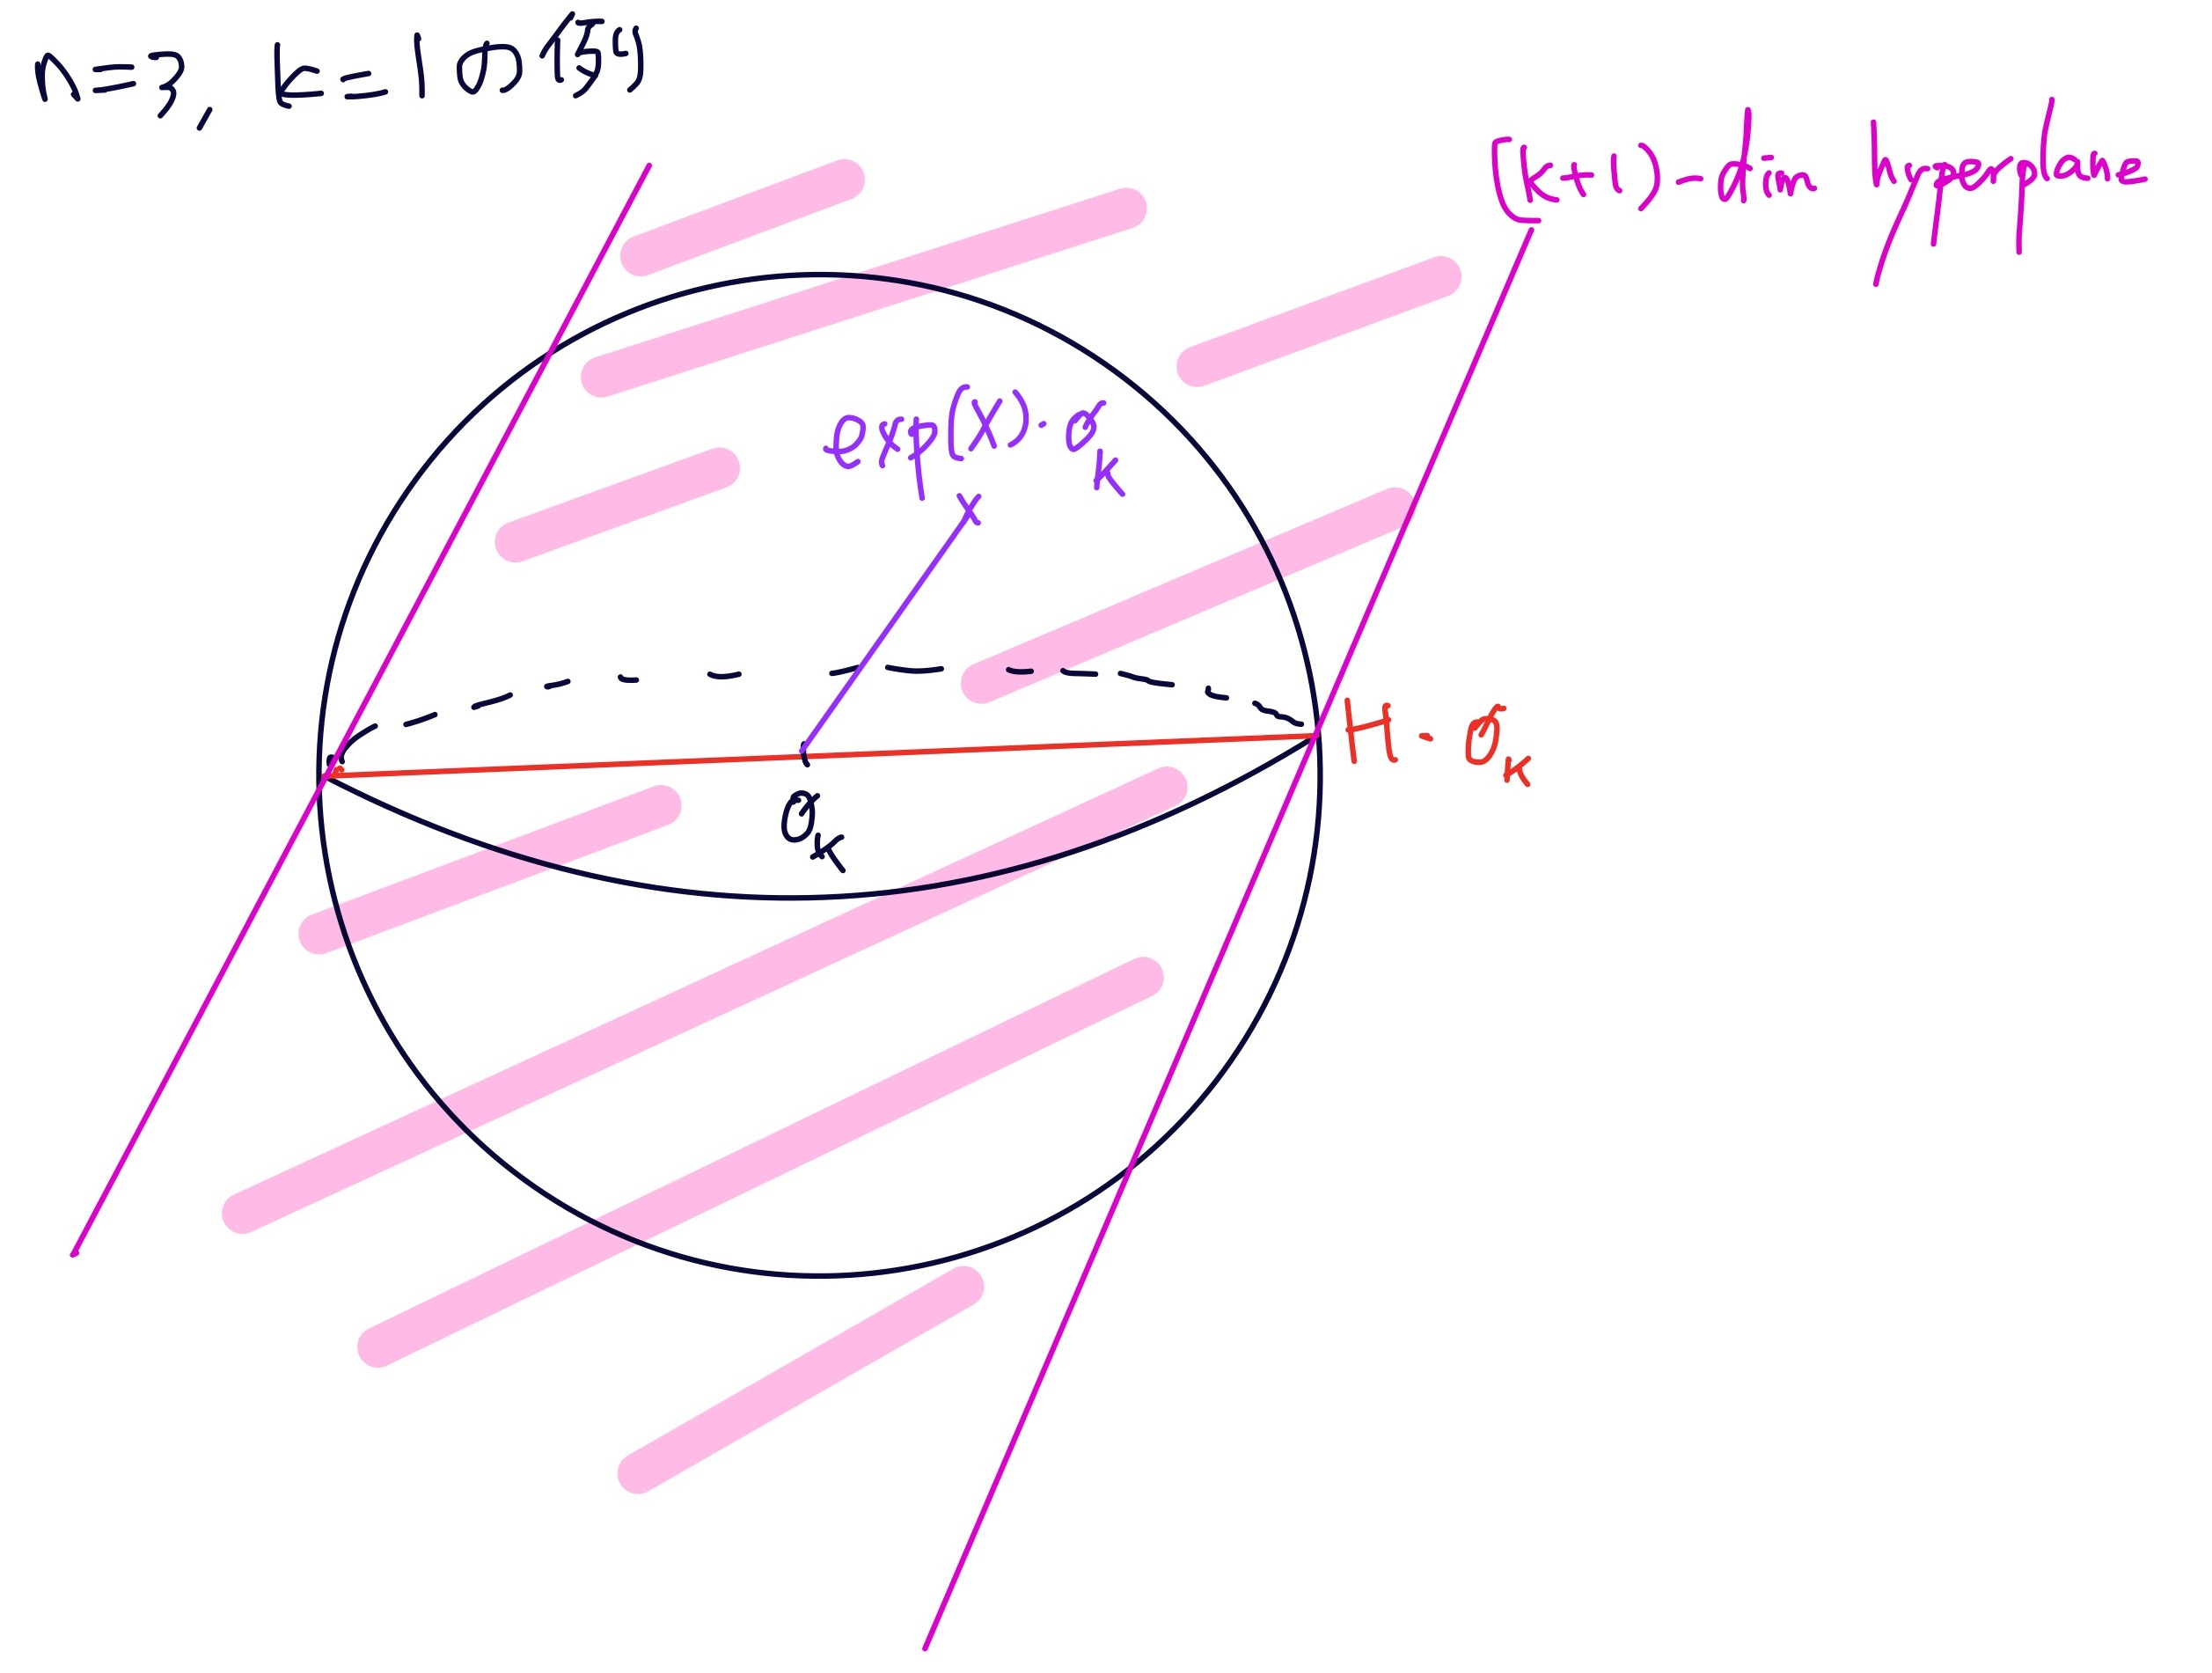
\includegraphics[scale=0.1]{../graph/son1.jpg}
    \caption{}
    \label{fig:son1}
  \end{figure}
  
  この断面に現れるのは\Cref{fig:yosou-eg-1}と同じであるから,同様の計算により\Cref{cor:yosou-eg}を得る.
  
\end{pfwn}


\subsection{\Cref{yosou:1121} の観察: \Cref{yosou:1121}の仮定を外した場合の成り立たない例}

\Cref{yosou:1121}と次の\Cref{yosou:1121-2}は同値である.
\begin{yosou}\label{yosou:1121-2}

  $\pe_{H,\bdd} = \{X\in \pe\mid [X,(\ha\cap\pe)]\neq \{0\} \text{ あるいは } X\perp (\ha\cap\pe)\text{ である.}  \}  $
  
\end{yosou}

ここで似た予想として次の$\ha\cap\pe$を$\ha$に置き換えた予想が立てられる.
\begin{yosou}\label{yosou:1101}
  $\pe_{H,\bdd} = \{X\in \pe\mid  [X,\ha]\neq \{0\} \text{ あるいは } X\perp \ha \text{ である.}\}  $
\end{yosou}

しかし\Cref{yosou:1101}には反例が存在する.
\begin{lem}\label{lem:1118-main}
  $G = \SL(3,\real) $,$Y_1\defeq \diag(1,1,-2)$,$Y_2 \defeq \begin{pmatrix}
    0 & 1 & 0\\
    -1 & 0 & 0 \\
    0 & 0 & 0
  \end{pmatrix}$,\\
  $\ha = \real Y_1 \oplus \real Y_2 $,$X = \diag(1,0,-1) $に対し,$[X,\ha] \neq \{0\} $であるが$Y(\real X) = \real Y_1 $であり,非有界である.
\end{lem}

\begin{calcof}{\Cref{lem:1118-main}}

  $\ha$は可換Lie環であり,$\ge = \slie(3,\real) $のCartan対合$\theta W \defeq -\trans{W} $に対し$\ha = \theta \ha$である.

  $[X,\ha]\neq 0 $は,$[X, Y_2] \neq 0$より従う.

  ここで$Z_1\defeq \diag(1,-1,0)\in \per{\ha}\cap \pe $であり,任意の$t\in \real$に対し,$e^{2tX} = e^{tY_1}e^{tZ_1} $であるから,$Y(\real X) = \real Y_1 $となり,\Cref{lem:1118-main} が示された.
  
\end{calcof}

\Cref{lem:1118-main}において$X$と$\ha$は,$[X,\ha] \neq \{0\} $だが$[X,(\ha\cap \pe)] = \{0\}$かつ$X\not\perp (\ha\cap \pe) $となるように取った.  

つまり\Cref{yosou:1101}の右辺を次の\Cref{yosou:1101-2}のように少し弱めても\Cref{lem:1118-main}はその反例になっている.
\begin{yosou}\label{yosou:1101-2}
  $\pe_{H,\bdd} = \{X\in \pe\mid  [X,\ha]\neq \{0\} \text{ あるいは } X\perp (\ha\cap\pe) \text{ である.} \}  $
\end{yosou}
